\documentclass[a4paper,12pt]{article}
\usepackage[czech]{babel}
\usepackage[utf8]{inputenc}
\usepackage{graphicx}
\usepackage[absolute,overlay]{textpos} % Додає можливість абсолютного позиціонування

\begin{document}

% Титульна сторінка
\begin{titlepage}
    \centering
    \vspace*{\fill}
    {\LARGE \textbf{Ratatouille}}\\[0.3cm]
    Meal Organizer\\[1.5cm]
    Členové týmu:\\[0.5cm]
    Bilyk Vladyslava - kapitán \\
    \texttt{xbilyk03} \\[0.5cm]
    Kucher Maryna \\
    \texttt{xkuche01} 
    \vspace*{\fill}
\end{titlepage}

\newpage

\section*{Uživatelský průzkum a specifikace}

\subsection*{Popis aplikace}
    Moderní rytmus života nás nutí neustále hledat způsoby, jak efektivně hospodařit s časem a zdroji. Bez jasného plánu je obtížné kontrolovat výdaje: nakupujeme příliš mnoho, zapomínáme, co už máme, a utrácíme peníze za produkty, které se mohou zkazit, než je stihneme použít. Rozhodli jsme se vytvořit aplikaci, která pomáhá tyto problémy řešit. Usnadňuje uspořádání všech produktů, které již doma máte, plánování jídel na konkrétní dny, vytváření podrobných nákupních seznamů, sledování, kolik peněz utratíte za jídlo, a dokonce i kontrolu data expirace produktů. Tento přístup umožňuje nejen ušetřit čas a peníze, ale také diverzifikovat vaši menu.

\subsection*{Cílová skupina, pro kterou je program určen}
    Lidé, kteří si rádi organizují svůj život, věk: starší 16 let.
    


\subsection*{Požadavky uživatele}
\begin{itemize}
    \item Závěr z rozhovoru s uživatelem od Kucher Maryny
    \begin{itemize}
        \item Dotazovaný je osmnáctiletý člověk, který začal žít sám a rád využívá aplikace pro organizaci každodenních úkolů
        \item Uživatel potřebuje pohodlnou a srozumitelnou aplikaci, která mu pomůže organizovat zásoby jídla, plánovat jídelníček na několik dní dopředu a ušetřit čas při rozhodování, co vařit každý den.
        Uživatel by rád měl možnost automaticky sestavit menu na základě dostupných produktů a receptů, které si sám vybral. Chce mít možnost snadno přidávat nové položky, sledovat, co je skladem, a kontrolovat datum spotřeby produktů.
        Důležitou funkcí by měla být také možnost rychlého vytvoření nákupního seznamu podle plánovaných jídel nebo chybějících produktů. Uživatel by uvítal, kdyby aplikace dokázala zobrazit přibližné náklady na nákup a, ideálně, umožnila sledovat výdaje za určité období.
    \end{itemize}
    \item Závěr z rozhovoru s uživatelem od Bilyk Vladyslavy
    \begin{itemize}
        \item Byl proveden rozhovor s osobou, která pravidelně vaří pro celou rodinu a potřebuje pomocníka pro plánování jídel a nákupů potravin.
        \item Závěr z rozhovoru: Uživatel by si přál mít v programu rozvrh/kalendář jídel, aby měl před sebou plán, co bude třeba připravit na následující dny. V seznamu dostupných potravin by chtěl označit základní potraviny (jako je sůl, cukr, máslo, rýže atd.), a když by tyto potraviny došly, obdržet upozornění. Dále by ocenil upozornění, když nebudou k dispozici potraviny pro jídlo přidané do kalendáře. Zajímala by ho také funkce doporučení jídel, která je možné připravit z dostupných potravin. Z dalších přání: Uživatel by rád dostával upozornění z kalendáře před svátky a přidával do nákupního seznamu speciální produkty pro svátky, například alkohol nebo dort.
    \end{itemize}
    \item Závěr týmu
    \begin{itemize}
        \item Závěr
    \end{itemize}
    \item Statistika odpovědí:
    % \begin{figure}[h!]
    %     \centering
    %     \includegraphics[width=0.5\textwidth]{cesta_do_фото}
    %     \caption{Popis obrázku}
    % \end{figure} % фото статисктики квізу
\end{itemize}

\section*{Průzkum existujících řešení}

\subsection*{Seznam aplikací. Pro a proti pro každou aplikaci}
\begin{itemize}
    \item \textbf{Mealime} : aplikace nabízí velkou databázi receptů s podrobným popisem vaření, možnost vytvoření nákupního seznamu.
    \begin{itemize}
        \item Výhoda :  Automatické vytváření nákupního seznamu. Možnost vařit s obrazem kroků receptu v reálném čase. Schopnost vytvářet si vlastní recepty nebo používat ty navržené.
        \item Nevyhoda : aplikace neposkytuje možnost ovládat seznam produktů, které jsou doma. Naplánované recepty nejsou propojeny s kalendářem.
    \end{itemize}
    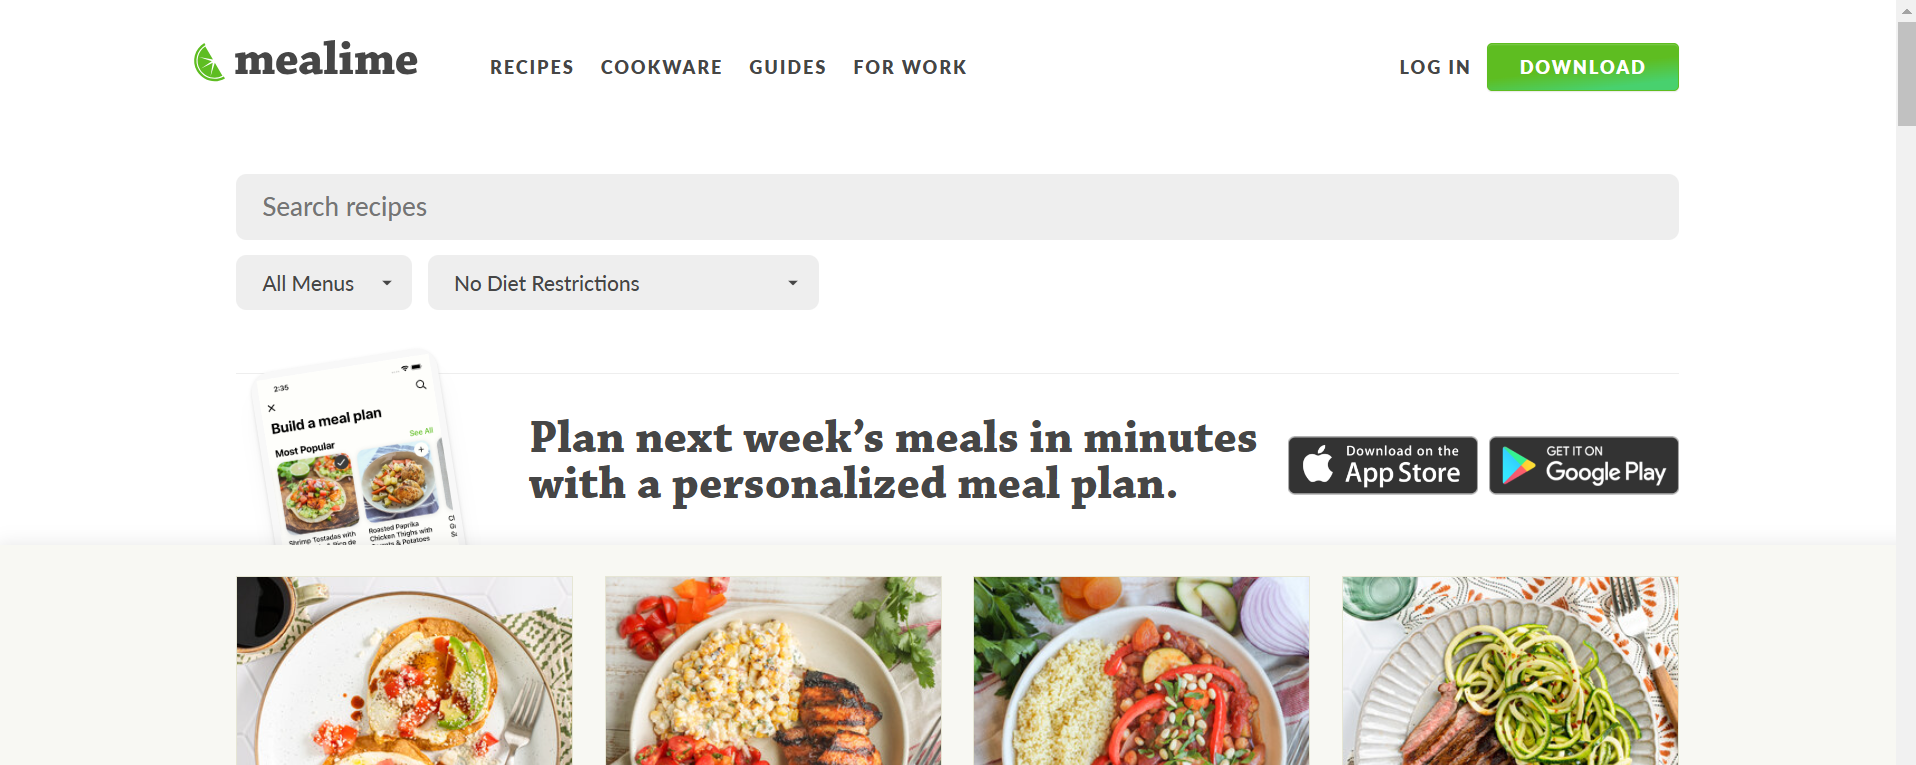
\includegraphics[width=0.9\textwidth]{mealime.png}
    

    \item \textbf{Meal planner grocery list} : Aplikace má kalendář s plánem menu, nákupním seznamem a seznamem s potravinami doma.
    \begin{itemize}
        \item Výhoda : Schopnost vytvářet pravidla jako „Pondělí je kuřecí den“. Schopnost přidat zdrojové odkazy na vlastní recepty.
        \item Nevyhoda : Nedostatek automatizace při vytváření nákupního seznamu (po naplánování jídla je nutné přidat produkt do nákupního seznamu). Chybí možnost plánování jídla mimo domov.  Aplikace neposkytuje možnost sledovat datum expirace produktů
    \end{itemize}
    \begin{center}
         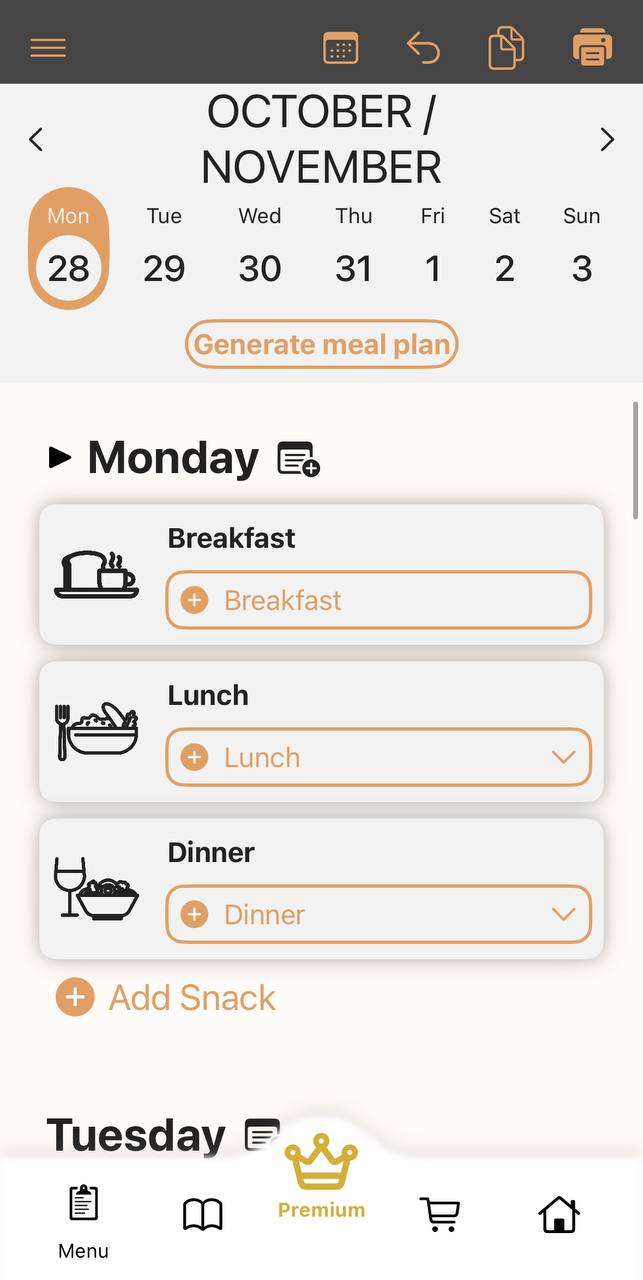
\includegraphics[width=0.35\textwidth]{grocerylist.png} % Шлях до зображення
    \end{center}
    
    \item \textbf{Daily Meal planner}
    \begin{itemize}
        \item Výhoda: V programu lze rozdělit přidané pokrmy na snídani, oběd a večeři. K dispozici je statistika spotřebovaných pokrmů za období, například posledních 30 dnů. Pokrmy jsou rozděleny do kategorií, z nichž každá je označena vlastní barvou, která se zobrazuje u pokrmu v kalendáři. K pokrmům lze přidat odkaz na web s receptem.
        \item Nevyhoda: Seznam produktů se nevyplňuje automaticky - uživatel musí vše zadávat ručně. Není také možné vést seznam produktů, které má uživatel k dispozici. Při zaplnění dne kalendáře pokrmy lze vytvořit nový pokrm a přidat ho do vybraného dne, například na snídani, ale nelze přidat žádné další informace kromě názvu pokrmu.
    \end{itemize}
   \begin{center}
        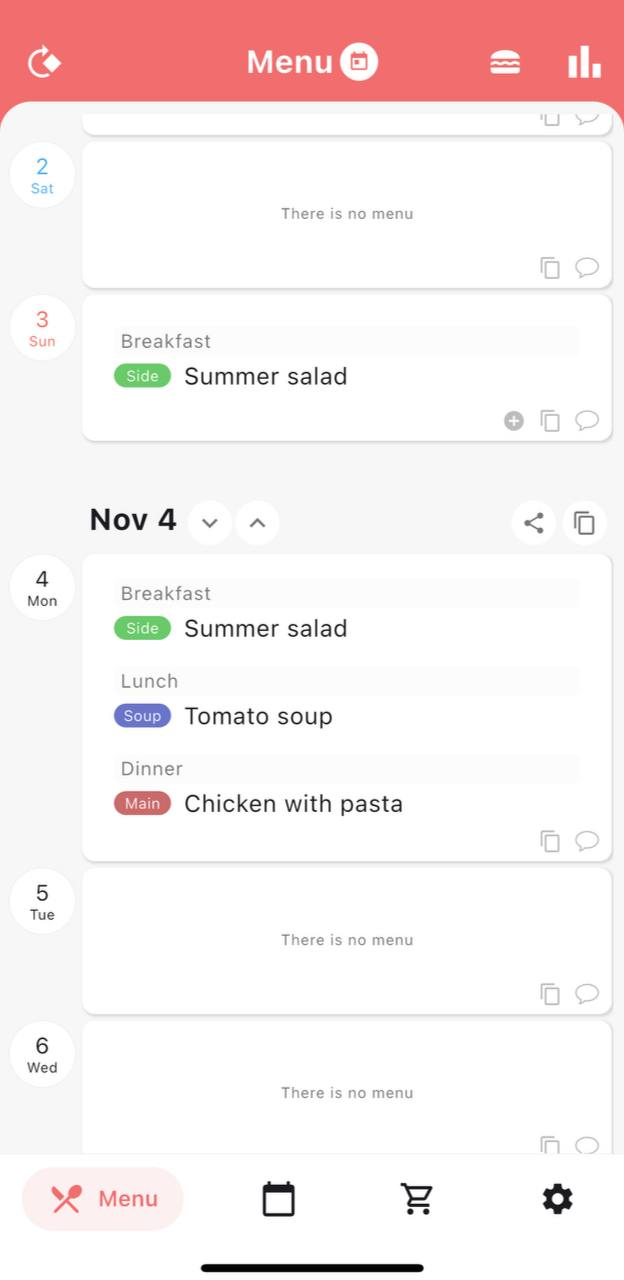
\includegraphics[width=0.3\textwidth]{Meal.jpg}
    \end{center}
    \item \textbf{Eatwell101}
    \begin{itemize}
        \item Výhoda: Program již obsahuje databázi s více než 3000 pokrmy, u nichž jsou uvedeny ingredience, recept, kalorická hodnota a další užitečné informace. Při přidání pokrmu do kalendáře se potřebné ingredience automaticky přidávají do seznamu produktů. Kromě přidání pokrmu do kalendáře je také možné uložit oblíbené pokrmy do vlastních receptů.
        \item Nevyhoda: Kalendář je určen pouze na týden, bez specifikace dnešního data. Není možné vytvářet vlastní recepty.
    \end{itemize}
    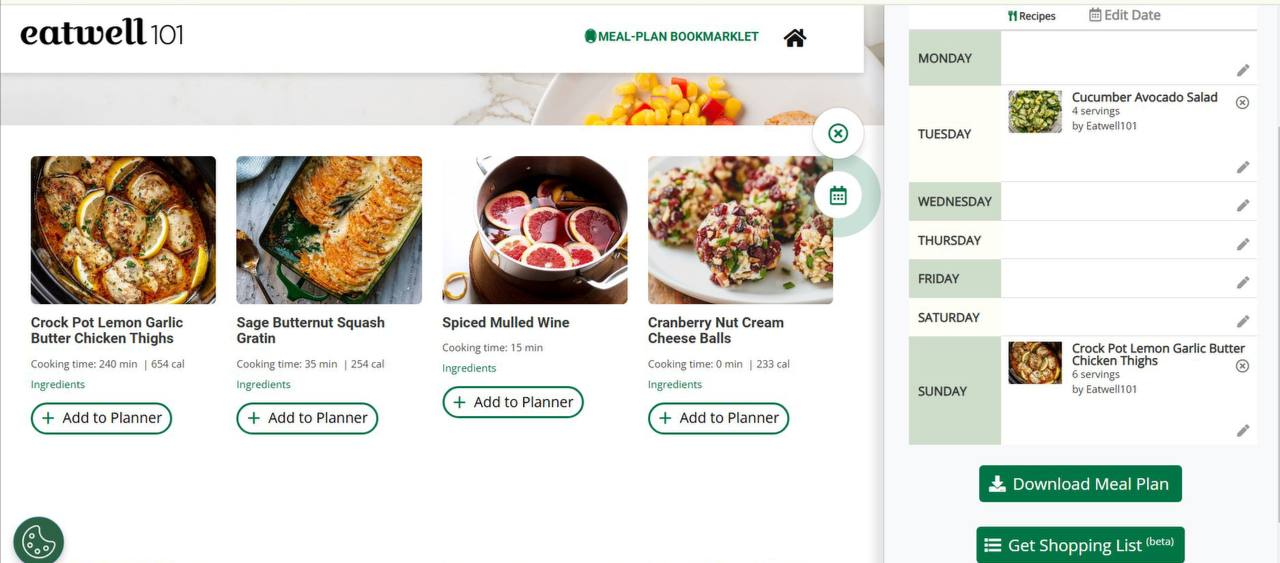
\includegraphics[width=0.9\textwidth]{eatwell101.jpg}
    
\end{itemize}


\subsection*{Závěry průzkumu}
\begin{itemize}
    \item Vyvození 3 inspirací/ponaučení pro návrh aplikace.
\end{itemize}

\subsection*{Popis požadované aplikace}
\begin{itemize}
    \item Popis aplikace: Klíčové funkce a části frontendu.
    \item Přehled aplikace a její funkčnosti.
\end{itemize}

\section*{Návrh}
\subsection*{Návrh GUI}
Pro frontend jsme zvolili React, protože je to jeden z nejoblíbenějších frameworků pro vývoj dynamických a interaktivních uživatelských rozhraní. 
React také poskytuje pohodlnou architekturu komponent, která usnadňuje vytváření, opětovné použití a údržbu jednotlivých prvků rozhraní. Rozdělili jsme naši aplikaci na nezávislé komponenty : Kalendář, ProductList, ShoppingList a DishesList.
\begin{center}
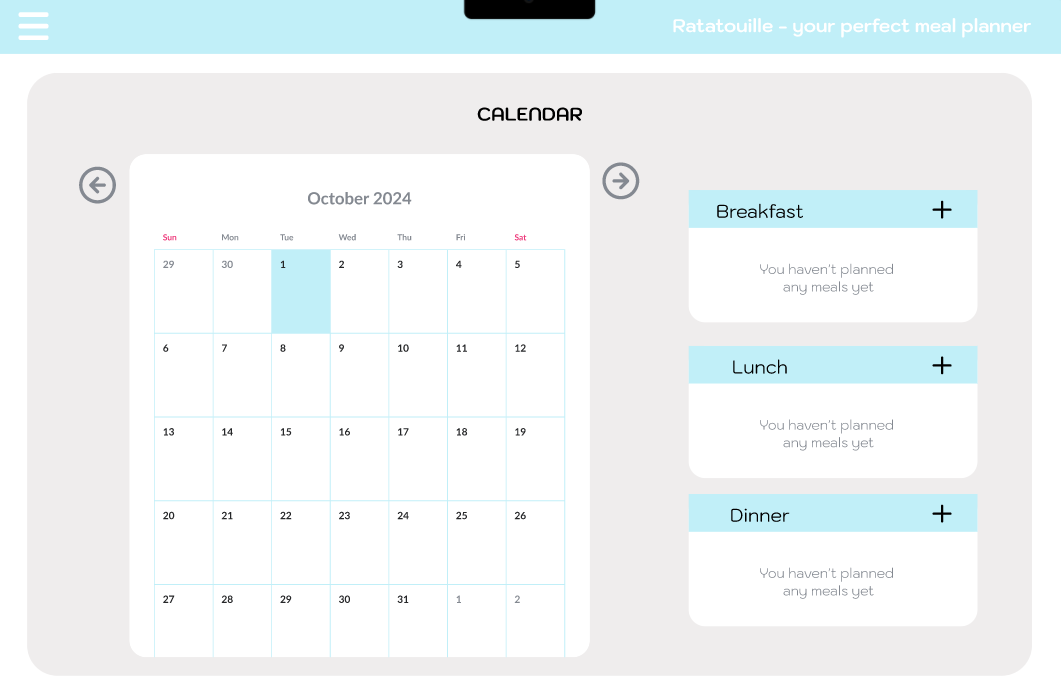
\includegraphics[width=0.7\textwidth]{figma_calendar.png}
\end{center}
ProductList – Tato komponenta zobrazuje seznam dostupných produktů a jejich krátký popis, které jsou připojeny k backendu a jsou přijímány prostřednictvím API požadavku. Díky Reactu lze seznam rychle aktualizovat bez nutnosti obnovovat celou stránku. Zobrazí se počet produktů, které se vejdou na obrazovku, je možné rolováním zobrazit další položky. Každý produkt lze snadno upravit nebo smazat.
\begin{center}
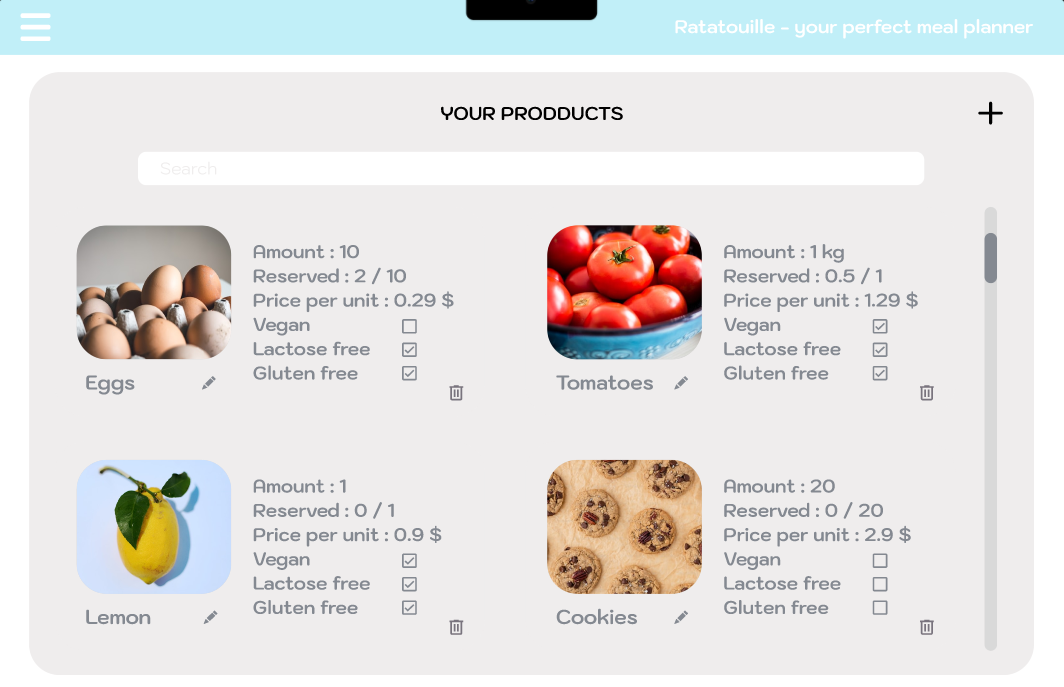
\includegraphics[width=0.7\textwidth]{figma_product.png}
\end{center}
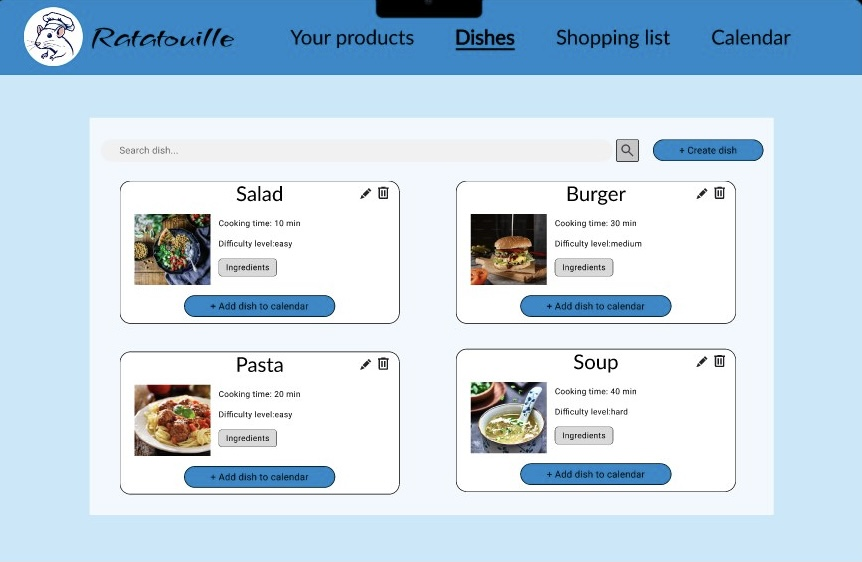
\includegraphics[width=0.9\textwidth]{dishes.JPG}

\begin{itemize}
    \item Popis  logické implikace navrženého GUI
\end{itemize}


\subsection*{Výběr technologií}
\begin{itemize}
    \item Popis technologii a zduvodneni
\end{itemize}

\subsection*{Návrh API k BE}
\begin{itemize}
    \item Popis  napojení FE na BE atd
\end{itemize}

\end{document}
